\section{Blind Attack}
\label{sec:blindattack}

In a real-world scenario, the key is typically unknown. Therefore we do not have any information whether our best candidate is correct or not. We need some rule to deduce so. Note that we can run ordinary AES encryption whenever we want to check our key candidate.

\begin{remark}
\label{rem:false}
	Especially note the attack against the \nth{0} byte using {\tt 3d} as a target and its last but one entry in Table \ref{tab:lintargets} -- here the incorrect candidate has a gap of almost $26\%$! It is actually the largest gap of an incorrect candidate ever seen among all targets and all bytes.
	%!% už neni, v jiných instancích tabulek viděno i víc (31.4)
	
	In our results, the target bits keep their original order (but reverse), therefore we can deduce the row $B$ generating the target in terms of $T_B$. Here it is the second row of matrix of multiplication by $\texttt{3d}\pmod{x^8+1}$, see Example \ref{ex:shiftmatrix}. Hence the row is $B = 01011110$.
	%!% neni! opravit a hlavně vočekovat že to tak opravdu je !!!
\end{remark}

For this reason, we studied our results deeper. The following section gives some of our remarks, next we suggest the blind attack itself in Section \ref{sec:subblindattack}


% ==============================================================================
% ===   R E M A R K S                                                        ===
% ==============================================================================

\subsection{Remarks}
\label{sec:remarks}

We processed our results of attack against {\tt KlinecWBAES} with $1024$ traces and displayed several statistics. Here we present some of them. Note that we filtered correct candidates with gap smaller than $5\%$ for this purpose.

\subsubsection{Leaking Bits}
	
	Remind that our trace is a bit-wise serialization of least significant bytes of memory addresses, hence we can identify which bit within that byte leaked -- simply by taking leaking position in trace modulo $8$ (note the difference from target bit). We noticed that it is not very well balanced, actually the \nth{0} and \nth{1} bits leaked slightly more and the \nth{3} bit did not leak at all! See histogram in Figure \ref{fig:leakbithist}.
	
	\begin{figure}[h]
	\begin{center}
		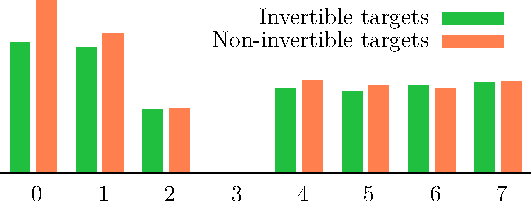
\includegraphics{figures/leak_bit/plot.pdf}
		\caption{Number of leaks at each bit within trace modulo $8$.}
		\label{fig:leakbithist}
	\end{center}
	\end{figure}

\subsubsection{Leaks per Target}
	
	And now leaks per target. %!% remake: udělat všech nezávislejch 255 a počítat procentuelně (možností má 16, tak asi ne uplně histogram, ale spíš průměrnej počet leaků na target a nák otestovat uniformitu)
	% asi taky udělat víc útoků s různejma tabulkama ...
	%~ We repeated this attack against all key bytes using $1024$ traces and observed following:
	%~ \begin{itemize}
		%~ \item $12.6$ targets per byte were successful ($\blacksquare$) on average (without any limit on gap),
		%~ \begin{itemize}
			%~ \item the rest gave incorrect candidate ($\boxtimes$),
		%~ \end{itemize}
		%~ \item correct candidates had average gap of $37\%$ with standard deviation of $11\%$,
		%~ \item incorrect candidates had average gap of $13.5\%$ with standard deviation of $4.5\%$,
	%~ \end{itemize}
	%~ We used this information and repeated the attack with only $128$ traces while
	%~ \begin{itemize}
		%~ \item considering only candidates beyond $\mu_\textnormal{false}+3\sigma_\textnormal{false} = 27\%$, we get
		%~ \begin{itemize}
			%~ \item $10.6$ successful targets on average,
			%~ \item no false positive i.e.\ incorrect candidates are filtered out.
		%~ \end{itemize}
	%~ \end{itemize}
	
	\ldots will be changed. Makes no sense
	
	\begin{figure}[h]
	\begin{center}
		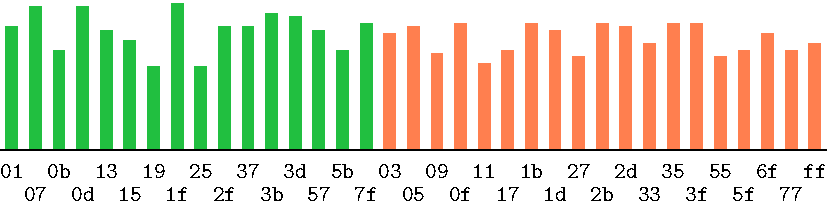
\includegraphics{figures/leak_target/plot.pdf}
		\caption{Number of leaks with each target. The number was doubled at {\tt 11}, {\tt 33} and {\tt 77}, fourtupled at {\tt 55} and eighttupled at {\tt ff} to fit the scale.}
		\label{fig:leaktargethist}
	\end{center}
	\end{figure}

\subsubsection{Using Less Traces}
	
	Note that once we use less traces, we usually do not find the correct candidate on the tail (as mentioned in Note \ref{note:tailrank}). Some results \ldots %!% results


% ==============================================================================
% ===   B L I N D   A T T A C K                                              ===
% ==============================================================================

\subsection{Blind Attack}
\label{sec:subblindattack}

\begin{note}
	This section only applies previous observations on a heuristic basis, there is no guarantee that our approach is the best.
\end{note}

We suggest to use less traces and repeat the attack with several targets. Even though we can hardly exploit the observation about candidates on the tail from Note \ref{note:tailrank}, it appears to be more robust and efficient to use several targets and sum the values of their respective best candidates unless filtered.

\ldots


% We rather suggest the following:
%~ \begin{enumerate}
	%~ \item pick a target, %!% Chi-square test of uniformity, pick random
	%~ \item attack using $256$ traces
%~ \end{enumerate}

%~ Therefore, in case of blind attack (i.e.\ no knowledge of actual key), we suggest to use less traces, but keep changing the target until the maximal gap exceeds $27\%$, then we accept that candidate. This is likely to happen soon since $10.6$ out of $16$ targets succeed on average.

% psal já / Teuwen:
%~ > I only wonder about the reasoning why Karroumi is more than Chow since
%~ > it seems to have been shown to be equal (based on what I wrote in my
%~ > previous email).
%~ 
%~ Well I've no problem to break completely Chow with standard DCA so there
%~ is something a bit more in Karroumi. Obviously not enough to make it
%~ robust enough...
